\section{Software: Samurai}
\label{sec:Samurai:software}



\begin{table}[h!]
    \centering
    { \setlength{\parindent}{0pt}
    \def\arraystretch{1.25}
    \arrayrulecolor{numpexgray}
    {\fontsize{9}{11}\selectfont
    \begin{tabular}{!{\color{numpexgray}\vrule}p{.4\textwidth}!{\color{numpexgray}\vrule}p{.6\textwidth}!{\color{numpexgray}\vrule}}
        \rowcolor{numpexgray}{\rule{0pt}{2.5ex}\color{white}\bf Field} & {\rule{0pt}{2.5ex}\color{white}\bf Details} \\
        \rowcolor{white}\textbf{Consortium} & \begin{tabular}{l}
IP Paris\\
\end{tabular} \\
        \rowcolor{numpexlightergray}\textbf{Exa-MA Partners} & \begin{tabular}{l}
CEA\\
IPP\\
\end{tabular} \\
        \rowcolor{white}\textbf{Contact Emails} & \begin{tabular}{l}
Loic Gouarin\\
\end{tabular} \\
        \rowcolor{numpexlightergray}\textbf{Supported Architectures} & \begin{tabular}{l}
CPU Only\\
\end{tabular} \\
        \rowcolor{white}\textbf{Repository} & \href{https://github.com/hpc-maths/samurai}{https://github.com/hpc-maths/samurai} \\
        \rowcolor{numpexlightergray}\textbf{License} & \begin{tabular}{l}
OSS::BSD\\
\end{tabular} \\
        \rowcolor{white}\textbf{Bottlenecks roadmap} & \begin{tabular}{l}
B10 - Scientific Productivity\\
B11 - Reproducibility and Replicability of Computation\\
B6 - Data Management\\
B7 - Exascale Algorithms\\
\end{tabular} \\
        \bottomrule
    \end{tabular}
    }}
    \caption{Samurai Information}
\end{table}

\subsection{Software summary}
\label{sec:Samurai:summary}

samurai is an open source software package written in modern C++ (C++17 and soon C++20), enabling the representation of sparse Cartesian meshes with different levels of resolution in a compressed way, using an interval representation. Resolution refers to Cartesian cells of the same size. A set algebra is provided to manage the operators that can intervene between these meshes. These include intersections, unions, differences and translations.
It is then possible to attach scalar and vector fields to these meshes and perform operations on these fields. Access operators facilitate field manipulation according to resolution levels and coordinates.

This data structure can then be used to implement spatial and temporal schemes. The figure below shows the different layers involved in samurai. Some of them are currently being implemented.

\begin{figure}[h!]
    \centering
    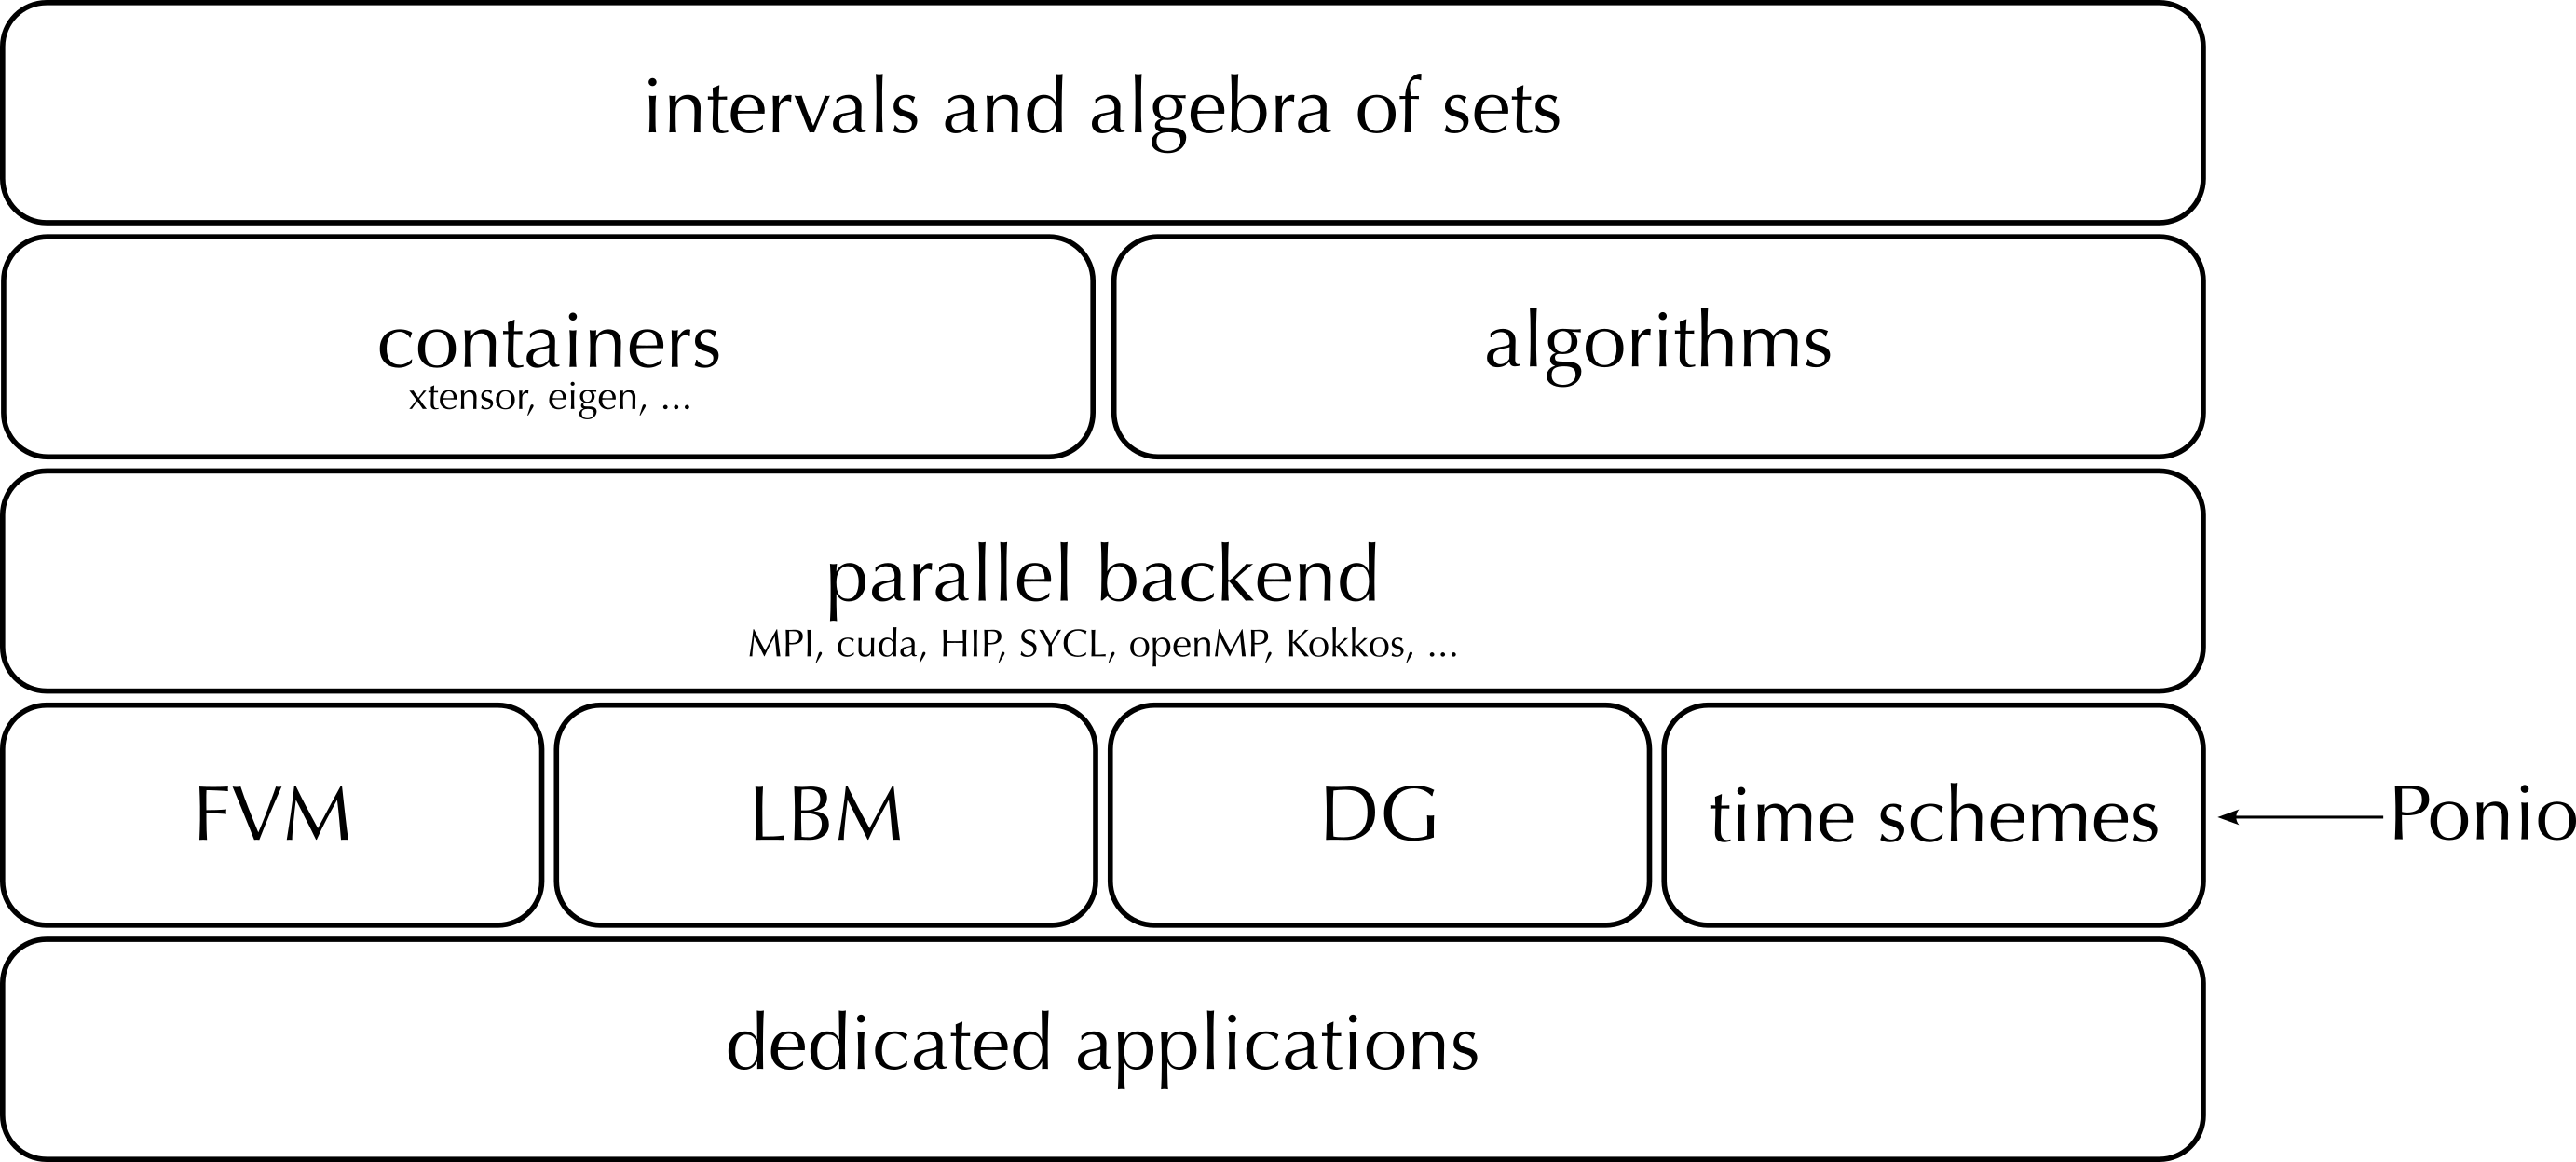
\includegraphics[width=0.8\textwidth]{graphics/samurai/samurai.png}
    \caption{Samurai architecture}
\end{figure}

\href{https://github.com/hpc-maths/ponio}{ponio} is also an open source software developed at the HPC@Maths team at CMAP (Ecole polytechnique). The aim of ponio is to provide a set of schemes in time for solving a whole collection of ODEs and PDEs. The simplest is the combination of an operator separation strategy and a method of line involving various classical time integrators like Runge-Kutta methods, or optimized one (RADAU5, ROCK4) and also splitting operator methods (IMEX, Strang splitting) ; the long-term objective is also to be able to tackle innovative adaptive code coupling techniques through an interface as well as classes of time-space coupled schemes (Lax-Wendroff, OSMP, time-space coupled IMEX with good asymptotic preserving and stability properties...).

The design principles of samurai are the following:
\begin{enumerate}
    \item Compress the mesh according to the level-wise spatial connectivity along each Cartesian axis.
    \item Achieve fast look-up for a cell into the structure, especially for parents and neighbors. This is particularly useful when utilizing numerical schemes such as Finite Volumes, \emph{etc.} on the hybrid mesh.
    \item Maximize the memory contiguity of the stored data to allow for caching and vectorization (contrarily to the $z$-curve).
    \item Facilitate inter-level operations which are common in many numerical techniques (\emph{e.g.} multiresolution).
    \item Allow for a time evolution of the hybrid mesh (\emph{via} AMR or multiresolution)  efficiently.
    \item Give the possibility of writing numerical schemes in a transparent way as one were on a uniform mesh.
\end{enumerate}

To give an overview of the compression capabilities of samurai, the following table shows the number of cells needed to represent a Cartesian mesh defined by the simple-2d example found in the p4est library (\cite{burstedde_p4est_2011}).

\begin{figure}[h!]
    \centering
    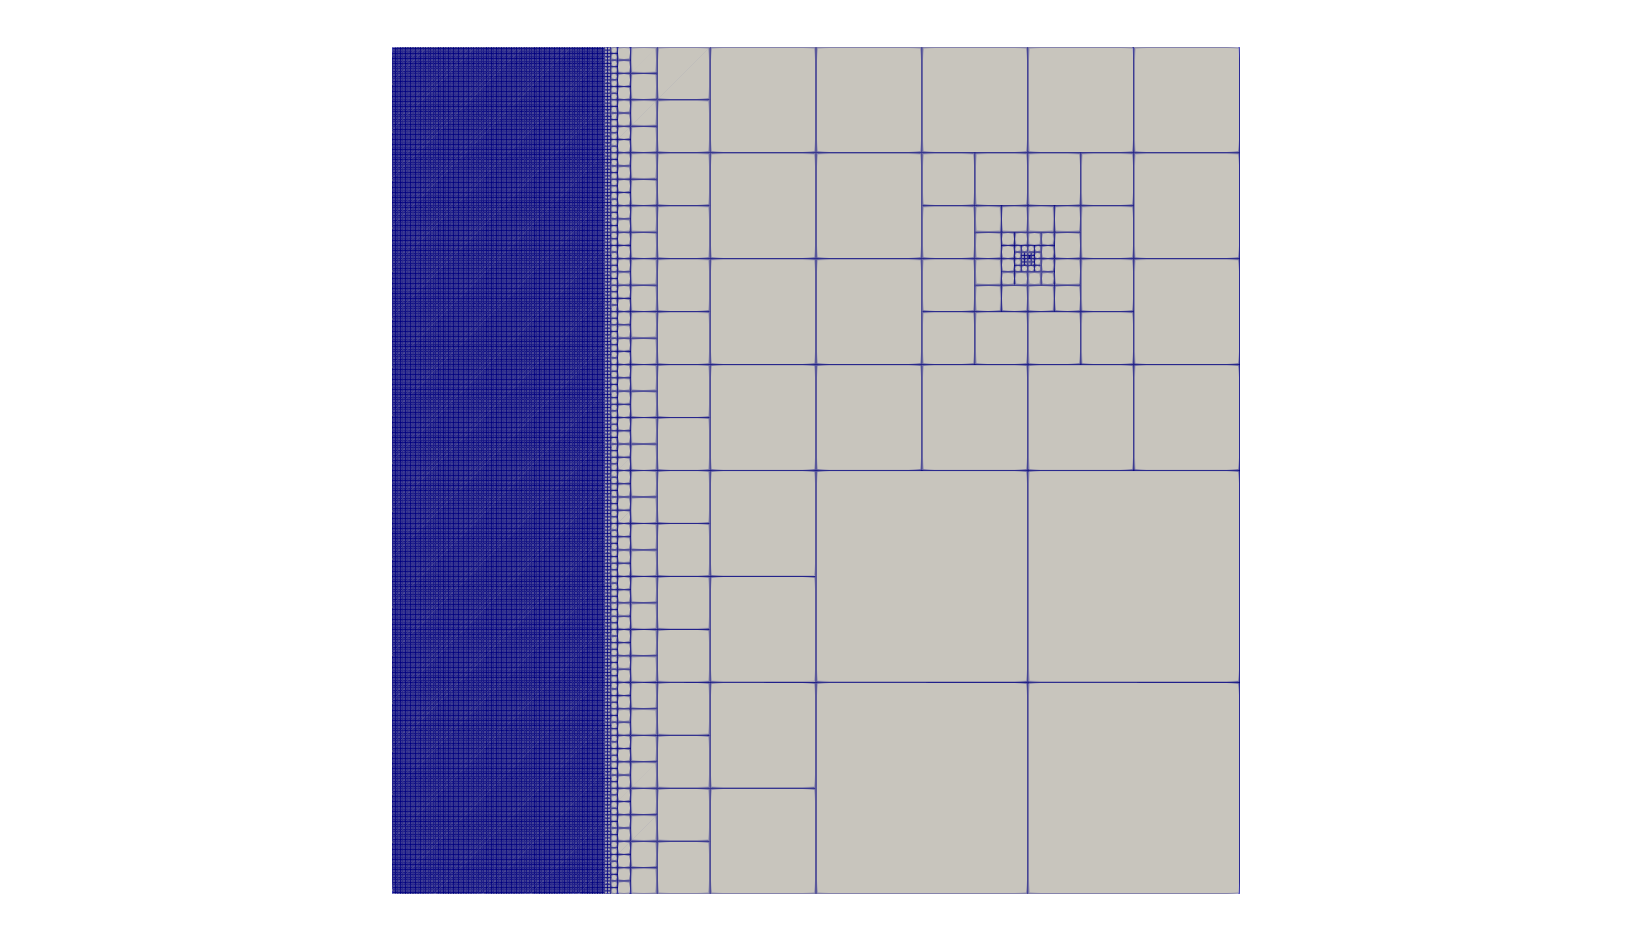
\includegraphics[width=0.8\textwidth]{graphics/samurai/p4est_3.png}
    \caption{simple-2d test from p4est library}
\end{figure}

\begin{table}[h!]
    \centering
    \rowcolors{2}{numpexlightergray}{white}
    \begin{tabular}{llllll}
        \textbf{Level} & \textbf{Num. of cells} & \textbf{p4est} & \textbf{samurai (leaves)} & \textbf{samurai (all)} & \textbf{ratio} \\
        \hline\hline
        9 & 66379 & 2.57 Mb & 33.68 Kb & 121 Kb & 21.24 \\
        10 & 263767 & 10.25 Mb & 66.64 Kb & 236.8 Kb & 43.28 \\
        11 & 1051747 & 40.96 Mb & 132.36 Kb & 467.24 Kb & 87.66 \\
        12 & 4200559 & 163.75 Mb & 263.6 Kb & 927 Kb & 176.64 \\
        13 & 16789627 & 654.86 Mb & 525.9 Kb & 1.85 Mb & 353.98 \\
        14 & 67133575 & 2.61 Gb & 1.05 Mb & 3.68 Mb & 709.24 \\
    \end{tabular}
\end{table}

\subsection{Purpose}
\label{sec:Samurai:purpose}

Based on this new data structure, samurai's objective is to be able to easily describe AMR mesh adaptation methods with a heuristic refinement criterion, or multiresolution methods based on a wavelet base decomposition. Multiresolution, although more complicated to implement, offers greater robustness than AMR methods, since the refinement criterion is based solely on the calculation of a detail derived from the wavelet decomposition. It therefore provides finer control over the error made between the fine solution everywhere and the adapted solution whatever the physical problem studied.

Block-based AMR methods have good memory contiguity thanks to their patch-based hierarchical data structure. This makes it possible to use the vectorization of modern processors. However, to be effective, the patches need to be large enough. It is therefore possible to refine more than necessary.

Cell-based AMR methods lose this memory contiguity, as the mesh is now flattened. A tree-like data structure is therefore required. To restore good arithmetic intensity, it is customary to place cell blocks in the tree leaves. Here again, we refine more than is necessary.

In comparison, the samurai data structure maintains memory contiguity in one direction by using intervals. This is the same as with AMR block-based methods. This ensures that modern processors remain vectorized. What's more, the data structure allows refinement only where necessary. This means no more refinement than is necessary, while maintaining good arithmetic intensity. samurai therefore combines the advantages of the two previous data structures.

\subsection{Programming and Computational Environment}
\label{sec::Samurai:environment_capabilities}


The following table summarizes these aspects for Samurai, providing a  view of its programming and computational capabilities.

\begin{table}[h!]
    \centering
    {
    \setlength{\parindent}{0pt}
    \def\arraystretch{1.25}
    \arrayrulecolor{numpexgray}
    {\fontsize{9}{11}\selectfont
    \begin{tabular}{lp{.3\textwidth}p{.5\textwidth}}
        \rowcolor{numpexgray}{\rule{0pt}{2.5ex}\color{white}\bf Category}  & {\rule{0pt}{2.5ex}\color{white}\bf Details} & {\rule{0pt}{2.5ex}\color{white}\bf Description}\\
        \rowcolor{white}Languages  & \begin{tabular}{l}
C++\\
C++14\\
C++17\\
\end{tabular} & Programming languages and language standards supported by the software \\
        \rowcolor{numpexlightergray}Parallelism  & \begin{tabular}{l}
MPI\\
Multithread\\
\end{tabular} & Parallel computing methods and frameworks utilized by the software.\\
        \rowcolor{white}Data Formats  & \begin{tabular}{l}
HDF5\\
\end{tabular} & Data formats that the software can handle or produce.\\
        \rowcolor{numpexlightergray}Resilience  & \begin{tabular}{l}
None\\
\end{tabular} & Fault tolerance and recovery mechanisms employed by the software.\\
        \rowcolor{white}DevOps & \begin{tabular}{l}
Continuous Delivery\\
Continuous Integration\\
\end{tabular} & Outlines the development and operational practices including continuous integration, containerization, and testing methodologies.  \\
        \rowcolor{numpexlightergray}Packaging  & \begin{tabular}{l}
Other\\
\end{tabular} & Software packaging and distribution.\\
        \rowcolor{white}Testing  & \begin{tabular}{l}
Functional\\
Unit\\
Validation\\
Verification\\
\end{tabular} & Testing methodologies employed to ensure software quality and correctness.\\
        \rowcolor{numpexlightergray}Containerization  & \begin{tabular}{l}
None\\
\end{tabular} & Container technologies used to package and deploy the software.\\
        \rowcolor{white}Interfaces  & \begin{tabular}{l}
PETSc\\
\end{tabular} & List of software Samurai has interfaces with.\\
        \bottomrule
    \end{tabular}
    }}
    \caption{Samurai programming and computational environment}
\end{table}



\subsection{Mathematics}
\label{sec:Samurai:mathematics}

samurai provides a set of operators for working with Cartesian grids of varying resolutions. Two distinct categories of operators can be identified:

\begin{itemize}
\item Prediction operators are employed to calculate the value of a field on a fine grid based on the value of a field on a coarse grid.
\item Projection operators are used to determine the value of a field on a coarse grid by using the value of a field on a fine grid.
\end{itemize}

The aforementioned operators are currently defined for control volumes up to order 11. The size of the associated stencils is automatically accounted for by samurai. In a near future, the same operators will be defined for finite differences and discountinuous Galerkin methods.

It is thus possible to reconstruct the solution at any desired resolution level. This enables the solution to be found at the finest level, as well as calculations to be performed involving two different AMR meshes. To illustrate this purpose, we can imagine a case where one mesh is used to solve the Navier-Stokes equations, while another is employed to simulate the propagation of a pollutant via an advection equation, wherein the velocity is derived from the velocity provided by the Navier-Stokes equations. The first mesh is adapted using the velocity field, whereas the second mesh is adapted using the pollutant concentration.

In addition to these resolution-level operators, samurai provides an API for defining finite-volume operators that can be used for both explicit and implicit methods. The defined FVM operator available with samurai are

\begin{itemize}
    \item linear homogeneous operator
    \item linear heterogeneous operator
    \item non-linear operator
\end{itemize}

In the following, we will illustrate the use of samurai with a simple example of a linear homogeneous operator. The operator is a scalar Laplacian operator defined as follows:

Since we have

\begin{equation*}
\int_V \Delta u = \int_{\partial V} \nabla u\cdot \mathbf{n},
\end{equation*}

the flux function to implement is a discrete version of $\nabla u\cdot \mathbf{n}$.
Here, we choose the normal gradient of the first order, requiring a stencil of two cells.
This is enough to write the static configuration:

\begin{listing}[ht]
\begin{minted}[
    linenos,                % Line numbers
    fontsize=\scriptsize,        % Reduce font size
    bgcolor=bgcolor,        % Slightly gray background
    frame=lines,            % Delimiters around the code
    framesep=2mm,           % Space between code and frame
    rulecolor=\color{gray}, % Color of the frame
    breaklines              % Allow line breaks in long lines
  ]{cpp}
auto u = samurai::make_field<1>("u", mesh); // scalar field

using cfg = samurai::FluxConfig<SchemeType::LinearHomogeneous,
                                1,            // output_field_size
                                2,            // stencil_size
                                decltype(u)>; // input_field_type
\end{minted}
\end{listing}

Now, denoting by $V_L$ (left) and $V_R$ (right) the stencil cells and $F$ their interface, the discrete flux from $V_L$ to $V_R$ writes

\begin{equation*}
    \mathcal{F}_h(u_h)_{|F} := \frac{u_R-u_L}{h},
\end{equation*}

where $u_L$ and $u_R$ are the finite volume approximations of $u$ in the respective cells, and $h$ is the cell length.
%Referring to formula :eq:`linear_comb`, the coefficients in the linear combination of $(u_L, u_R)$ correspond to $(-1/h, 1/h)$.
The flux function then writes:

\begin{listing}[ht]
    \begin{minted}[
        linenos,                % Line numbers
        fontsize=\scriptsize,        % Reduce font size
        bgcolor=bgcolor,        % Slightly gray background
        frame=lines,            % Delimiters around the code
        framesep=2mm,           % Space between code and frame
        rulecolor=\color{gray}, % Color of the frame
        breaklines              % Allow line breaks in long lines
      ]{cpp}
samurai::FluxDefinition<cfg> gradient([](double h)
{
    static constexpr std::size_t L = 0; // left
    static constexpr std::size_t R = 1; // right

    samurai::FluxStencilCoeffs<cfg> c;
    c[L] = -1/h;
    c[R] =  1/h;
    return c;
});
\end{minted}
\end{listing}

First of all, remark that we have declared only one flux function for all directions.
We could have written as many functions as directions:
they would have been identical, except that we would have replaced the name of the constants
\verb!L=0, R=1! with \verb!B=0, T=1! (bottom, top) and \verb!B=0, F=1! (back, front) to better reflect the actual direction currently managed.
The indexes 0 and 1 actually refer to the configured stencil.
In this case, no particular stencil has been defined, so the default ones are used: in the x-direction of a 3D space,
it is \verb!{{0,0,0}, {1,0,0}}!, i.e. the current cell at index 0 (which we call \verb!L!) and its right neighbor at index 1 (which we call \verb!R!).

Finally, the operator must be constructed from the flux definition by the instruction

\begin{listing}[ht]
    \begin{minted}[
        linenos,                % Line numbers
        fontsize=\scriptsize,        % Reduce font size
        bgcolor=bgcolor,        % Slightly gray background
        frame=lines,            % Delimiters around the code
        framesep=2mm,           % Space between code and frame
        rulecolor=\color{gray}, % Color of the frame
        breaklines              % Allow line breaks in long lines
      ]{cpp}
auto laplacian = samurai::make_flux_based_scheme(gradient);
\end{minted}
\end{listing}

samurai uses lazy evaluation to have concise and readable equations. The following code snippet shows how to apply the operator to a field to solve the heat equation in implicit and explicit ways using backward Euler time scheme

\begin{listing}[ht]
    \begin{minted}[
        linenos,                % Line numbers
        fontsize=\scriptsize,        % Reduce font size
        bgcolor=bgcolor,        % Slightly gray background
        frame=lines,            % Delimiters around the code
        framesep=2mm,           % Space between code and frame
        rulecolor=\color{gray}, % Color of the frame
        breaklines              % Allow line breaks in long lines
      ]{cpp}
auto unp1 = samurai::make_field<1>("unp1", mesh);
if (explicit_scheme)
{
    unp1 = u - dt * laplacian(u);
}
else
{
    auto back_euler = id + dt * laplacian;
    samurai::petsc::solve(back_euler, unp1, u); // solves the linear equation   [Id + dt*Diff](unp1) = u
}
\end{minted}
\end{listing}

It can be observed that the implicit case is constructed and solved using PETSc.

These operators can then be used in adapted mesh refinement methods.

\subsection{Relevant Publications}
\label{sec:Samurai:publications}

Here is a list of relevant publications related to the software:

\begin{itemize}
    \item \cite{bellotti_multidimensional_2022}: this article explains how to use the adaptive multiresolution (MR) approach based on wavelets with lattice Boltzmann methods.
    \item \cite{bellotti_multiresolution-based_2022}: in this article, an error analysis is proposed. For the purpose of validating this error analysis, we conduct a series of test cases for various schemes and scalar and systems of conservation laws, where solutions with shocks are to be found and local mesh adaptation is especially relevant. Theoretical estimates are retrieved while a reduced memory footprint is observed.
\end{itemize}

\subsection{Acknowledgements}
\label{sec::Samurai:acknowledgements}

The software has been developed with the support of the following funding agencies and institutions:
\begin{itemize}
    \item \'Ecole polytechnique
    \item CNRS
    \item CIEDS
 \end{itemize}
